% THIS IS SIGPROC-SP.TEX - VERSION 3.1
% WORKS WITH V3.2SP OF ACM_PROC_ARTICLE-SP.CLS
% APRIL 2009
%
% It is an example file showing how to use the 'acm_proc_article-sp.cls' V3.2SP
% LaTeX2e document class file for Conference Proceedings submissions.
% ----------------------------------------------------------------------------------------------------------------
% This .tex file (and associated .cls V3.2SP) *DOES NOT* produce:
%       1) The Permission Statement
%       2) The Conference (location) Info information
%       3) The Copyright Line with ACM data
%       4) Page numbering
% ---------------------------------------------------------------------------------------------------------------
% It is an example which *does* use the .bib file (from which the .bbl file
% is produced).
% REMEMBER HOWEVER: After having produced the .bbl file,
% and prior to final submission,
% you need to 'insert'  your .bbl file into your source .tex file so as to provide
% ONE 'self-contained' source file.
%
% Questions regarding SIGS should be sent to
% Adrienne Griscti ---> griscti@acm.org
%
% Questions/suggestions regarding the guidelines, .tex and .cls files, etc. to
% Gerald Murray ---> murray@hq.acm.org
%
% For tracking purposes - this is V3.1SP - APRIL 2009

\documentclass{iitkthesis}
%\usepackage{algorithm2e}
%\usepackage{algpseudocode}
%\usepackage[pass,paperwidth=8.5in,paperheight=11in]{geometry}
%\usepackage[paperwidth=8.5in, paperheight=11in]{geometry}
%\newcommand{\commentSW}[1]{\textbf{SW --} \emph{#1} \textbf{-- SW}}

\begin{document}
%\pdfpagewidth=8.5in
%\pdfpageheight=11in

\title{Dialog-Based Location Unaware Wayfinding}
%\titlenote{(Does NOT produce the permission block, copyright information nor page numbering). For use with ACM\_PROC\_ARTICLE-SP.CLS. Supported by ACM.}}
%\subtitle{[Extended Abstract]
%\titlenote{A full version of this paper is available as
%\textit{Author's Guide to Preparing ACM SIG Proceedings Using
%\LaTeX$2_\epsilon$\ and BibTeX} at
%\texttt{www.acm.org/eaddress.htm}}}
%
% You need the command \numberofauthors to handle the 'placement
% and alignment' of the authors beneath the title.
%
% For aesthetic reasons, we recommend 'three authors at a time'
% i.e. three 'name/affiliation blocks' be placed beneath the title.
%
% NOTE: You are NOT restricted in how many 'rows' of
% "name/affiliations" may appear. We just ask that you restrict
% the number of 'columns' to three.
%
% Because of the available 'opening page real-estate'
% we ask you to refrain from putting more than six authors
% (two rows with three columns) beneath the article title.
% More than six makes the first-page appear very cluttered indeed.
%
% Use the \alignauthor commands to handle the names
% and affiliations for an 'aesthetic maximum' of six authors.
% Add names, affiliations, addresses for
% the seventh etc. author(s) as the argument for the
% \additionalauthors command.
% These 'additional authors' will be output/set for you
% without further effort on your part as the last section in
% the body of your article BEFORE References or any Appendices.
% \setcoguide{Prof. Bharat Lohani}
% setexguide{Prof. Stephan Winter}
% setcoguidedept{Department of Geoinformatics}
% setexguidedept{Department of Geomatics}

\author{Arbaz Khan}
\iitbdegree{Master of Technology}
\department{Computer Science and Engineering}
\rollnum{Y9227128}
\setguide{Prof Harish Karnick}
\setguidedept{Computer Science and Engineering}
\setcoguide{Prof Bharat Lohani}
\setexguide{Prof. Stephan Winter}
\setcoguidedept{Department of Geoinformatics}
\setexguidedept{Department of Geomatics}
\setexguideaff{University of Melbourne}
\dissertation
\maketitle
\makecertificate
\begin{abstract}
I plan to finalize the text of the abstract in the end of the writing.
%We also provide an insight into the complexity of the untackled problem of resolving the frame of reference.
\end{abstract}
\tableofcontents
\chapter{Introduction}
 \chapter{Problem Definition and Related Work}
 \section{Dialog Based Wayfinding Systems} 
Significant research has been done in the area of defining 
\cite{lovelace} and generating \cite{Dale,Habel,Maab,pattabhiraman} good 
quality route instructions which are specialized for human understanding. 
These models have evolved from those working on handcrafted data 
disseminating turn-by-turn instructions in a one-step-per-sentence 
mapping to the systems processing data from Geographic Information 
Systems (GIS) using visible features of the surroundings and generating 
compact and more human-like descriptions. Yet, most of these systems were 
one-way systems in which the instructions are provided in advance or 
even incrementally leading to poor comprehension and 
an inability to resolve ambiguities along the path. Owing to the 
benefits of a dialog system to respond to user queries and the possibility to 
react to inadequate or poorly understood instructions, research  
\cite{hurtig, jokinen, richter} had moved towards building dialog-driven 
wayfinding models. The major concern in these systems is to avoid 
overwhelming the user with too much information (or media) to avoid cognitive 
overload while giving enough detail to produce comprehensive and accurate 
descriptions preventing any ambiguities or confusions. Some \cite{richter} 
of these systems rely on purely speech-based interaction while others 
\cite{hurtig,jokinen} have used a multimodal interface which offers the user 
freedom to combine speech, pen and graphics based input. 
Although, multimodal systems do help a user to choose the preferred mode of
interaction and consequently result in better and disambiguated input signals
they compromise the main requirement of wayfinding assistance, which is, to 
reduce distractions while driving. 
Pure-auditory based route instructions help in minimizing the 
interference to driving and thus create no negative impact on reaction 
times \cite{srinivasaneffect}. 
 
At present, there are very few systems using just spoken 
dialogue for wayfinding. These systems can be classified into 
three categories depending on the target domain - indoor wayfinding, human
-machine interaction and outdoor wayfinding. The systems \cite{fongsurvey} 
based on human-machine interaction aim to facilitate the machine in 
execution of spatial tasks by providing route information and handling 
questions raised on detecting ambiguities. These tasks though 
certainly are similar to real world wayfinding assistance models in 
dialog structure and end goals but differ in the ability of their subjects. 
Humans follow subjective and non-uniform speed-patterns, instruction 
understanding behavior and conceptual memory models. 

For outdoor wayfinding, Janarthanam et. al. \cite{janarthanam} introduced 
a mobile dialogue application that combines GIS systems with spoken-
dialog to assist tourists in city navigation. It allows 
tourists to initiate tasks such as entity search (e.g. a museum or a 
restaurant), navigation assistance, entity inquiry and others. The 
proposed architecture is capable of fairly complex spoken-
dialog interaction (e.g., Take me to Hume) with the help of its semantic 
parser and  modules for natural language generation (NLG) and 
understanding (NLU). Richter et. al. \cite{richter} worked on generating 
context-based route instructions for outdoor wayfinding. Using a spoken 
dialog interface, the proposed conceptual model allows a user to tune the 
details of the route instructions from incremental turn-by-turn 
instructions to a more abstract set of instructions focussing upon 
destination descriptions. The model identifies and adapts to the wayfinder's 
spatial knowledge about the street network after deciding the prominence 
of a spatial entity derived from a hierarchy of visual, structural and 
cognitive features. Spoken-dialog systems for indoor wayfinding systems 
have not been built so far to the best of our knowledge. Cuay\'{a}huitl 
et. al.  \cite{heriberto} worked on a text-based dialogue system for indoor 
wayfinding which can respond to user queries on locations in a building. 
The authors claimed that a dialogue system for indoor wayfinding with 
only text-based interaction leads to very high overall scores of user 
satisfaction. Despite the fact that indoor settings are perfect for 
application of location-unawareness, yet none of these systems have  
attempted it and rely on certain location sensitivity (such as support 
for infrared and wireless media) in the end-device. Also, the relatively 
less emphasis on evolution of pure spoken-dialog systems can be 
understood owing to their limitations in poor speech recognition and 
unfulfilled linguistic expectations. 

In this work we try to overcome these limitations by setting up a cross-
lingual communication platform to convey non-ambiguous route instructions.
Furthermore, questions posed to the user for location tracking are 
such that the responses are recognisable speech commands 
(such as `yes',`no') and require only primitive speech processing. 
 \section{Evaluation Techniques}
Simulations in a virtual environment provide an important means for 
evaluation and improvement of real-world systems. Once the virtual 
environment is set-up, the next task is to identify the metrics for 
evaluating effectivenss of the system. The work done in this thesis is 
closely related to natural language generation (NLG), except that we focus 
only on the spatiotemporal content of the linguistics. Thus, the 
technique and metrics used for evaluating NLG systems are relevant in 
this context. For example, if the number of users who reach the target 
are fewer, it reflects poorly on the quality of the NLG and thus 
could be related to the underlying spatio-temporal content of the 
instructions. It is only recently that increasing effort has 
been put into evaluation of NLG systems. As Spanger et. al. \cite{spanger} 
point out, there can be two categories of methods to evaluate the 
effectiveness of an NLG system - intrinsic and extrinsic. \textit{
Intrinsic} methods compare the system with a benchmark/gold standard 
system, and \textit{extrinsic} methods use metrics like the number of 
mistakes made by the user while following the instructions \cite{young}. 

Further, research on evaluation of NLG tasks and investigation of issues 
has moved towards introducing shared task challenges \cite{give}. In this 
task the evaluation is assessed based on the performance of human users 
who follow the instructions of the NLG in a virtual environment with 
several rooms and corridors. The performance evaluation uses a set of 
objective as well as subjective measures. Objective measures include the 
distance travelled and time taken in reaching the goal as well as the 
number of instructions provided and the number of words per instruction. 
While, subjective measures provide a subjective rating of these 
instructions whether the instructions were useful. An interesting area of 
research \cite{GRUVE} then emerged which works on modelling navigation 
assistance with real world problems like uncertainty in location and 
noisy feedback signals from the user. These works exploit the utility of a 
virtual environment to eliminate the time and costs of real world 
experiments as well as provide a means to manipulate the environment 
targeting specific issues and context.

In this work, we move beyond the above mentioned virtual environments 
tested on humans. With the virtualization of the spatial environment, we also 
virtualize the user via driver modelling and use a set of goodness 
metrics to measure the effectiveness of the system. Independent works 
have been done in the area of simulating driver behavior to study traffic 
and accident patterns but none of these have been integrated into a 
testbed for wayfinding assistance.

%Since, in our case where no gold standard system is available and directly comparing the sytem to GPS would be unfair
%Simulations in a virtual environment provide an important means for evaluation and improvement of real-world systems.  
 %Performance evaluation on a task is the basic requirement to measure effectiveness of a natural language generation (NLG) system \cite{reiter}.  
 \chapter{Conceptual Model For Wayfinding}
We introduce our location-unaware wayfinding model through a generic 
spoken-dialog based model for wayfinding. This model can be transformed 
to a location-unaware wayfinding model by specializing the module 
structure. The aim of this model is to assist wayfinding tasks using 
natural language dialogues. The next section presents an architecture of 
the model. We propose a natural language independent communication 
protocol for conveying route-instructions.
 \section{Architecture}
The generic wayfinding model is designed to incorporate any linguistic 
structure and a predefined technique for user localization. It could 
be personalized for an user and should be able to identify and react to 
the context realizing the differences and constraints. The knowledge base 
behind is dynamically updateable to incorporate 
the changes in the spatial environment (such as broken road links, new 
buildings, etc). An architecture for the system realizing the requirements is 
shown in Figure \ref{fig:arc}. 
 \begin{figure}
\centering
%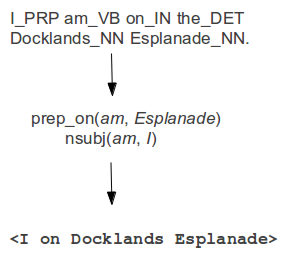
\includegraphics[width=0.5\textwidth]{phase1.png}
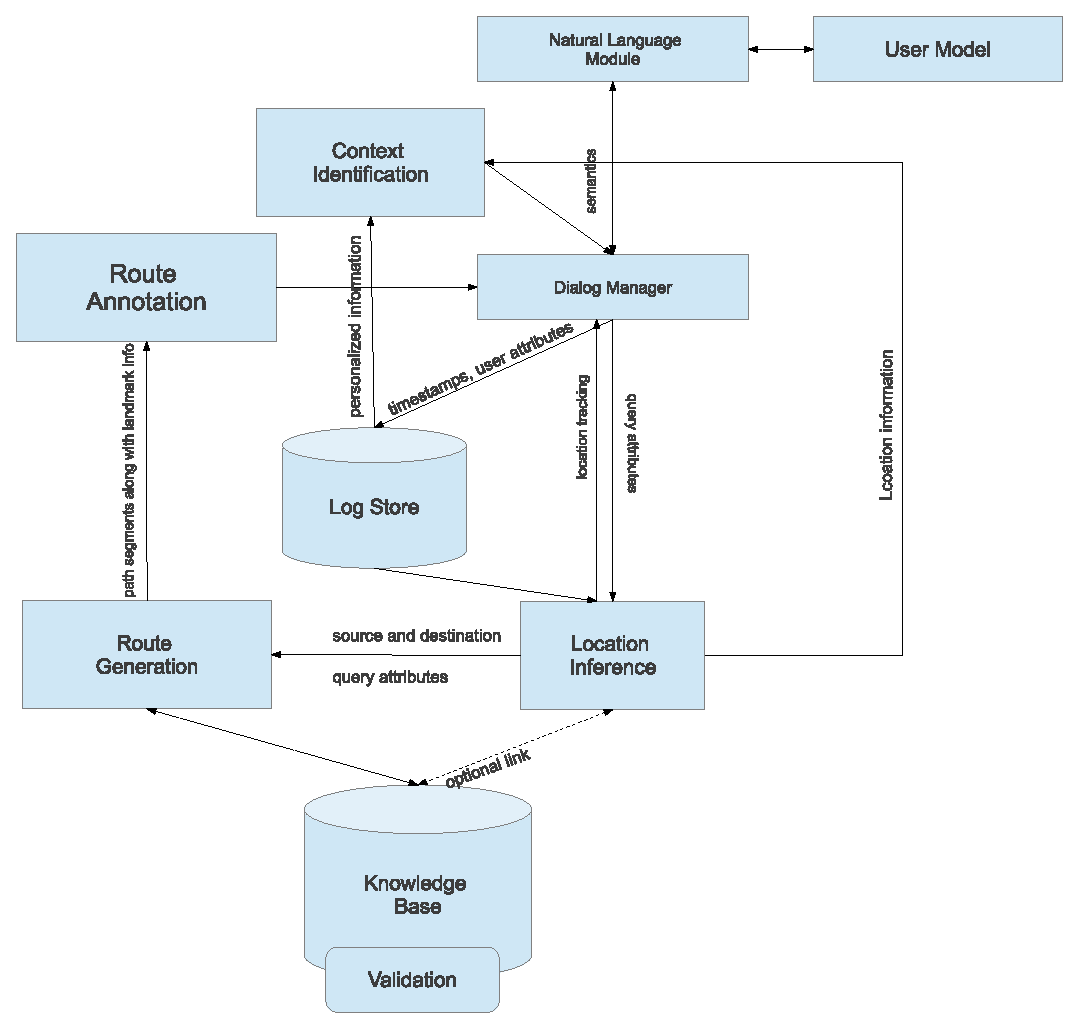
\epsfig{file=architecture.eps, height=4.2in, width=4.5in}
\caption{Architecture for a generic wayfinding model}
\label{fig:arc}
 \end{figure}
First, a \textit{user} (real human or artificial agent) requests for assistance 
to a destination. The \textit{Natural Language Module} parses the 
semantics of utterances, processes spatial information and records a new 
query into the system. Before route instructions are generated, it 
is necessary to locate the user (obtain the source location). Most of the 
wayfinding systems today use GPS systems for this purpose in an outdoor 
environment and wireless or infrared in indoor settings. Baus et. 
al. \cite{baus} introduced an adaptive model for localization that 
alternates between the different sensing technologies to overcome their 
individual limitations. For our system, we seek 
the user's location via dialog-based tracking, posing simple questions 
using features of a spatial environment. Nonetheless, we can abstract a 
module specifically for \textit{location inference} which either can work 
independently (by using sensors or receptors) or use the 
\textit{knowledge base} of the system for localization. Thus, the 
knowledge base stores a characterization of the complete spatial 
environment. It also stores the transportation network for target modalities 
(e.g., road links for vehicles, abstract spaces for pedestrians) and its 
relationship with the environment features (e.g., landmark-street 
association).

Once the information required to compute the topological route is 
collected, then the desired route is computed using query attributes 
(such as preferred route option like shortest route, scenic route, etc. 
and modality constraints like roads permissible for 4-wheelers). This 
computed route is passed on together with nearby landmark information for 
\textit{route annotation}. The route annotator processes the salience of 
the landmarks, removes redundant spatial relationships and fills up the 
spatial content of the route instructions. Besides operating on the 
processed information, the system is also sensitive to the context i.e. 
user attributes (such as modality, speed patterns) and location 
information. The context needs to be considered before generating natural 
language route instructions. With the help of contextual information, a 
decision is made by the \textit{dialog manager} on the delivery of route 
instructions to synchronize with when a user needs it. So, 
decisions like these make sure that turn instructions are temporally 
matched with an user's movement. The dialog manager also compiles the route 
instructions into a form understandable by the natural language module, 
which then serves to eventually fulfill the user request.
  \section{Communication Protocol}
In this section we introduce a communication protocol which allows
cross-lingual platform development. The protocol is targeted to deal with 
two kinds of scenarios - simple intersections and complex intersections. 
These latter scenarios deal with intersections having a 
large number of possible actions (more than 4) and tackling 
ineffectiveness of standard direction models. In similar 
work, Klippel \cite{klippel} introduced a formal representation of turn 
directions at decision points which could be chunked to produce better 
quality route instructions and could be tailored as per user preferences. 
But the formal theory model targets only simple intersections. Our 
approach is based on a similar notational representation of turn 
instructions but extends to complex intersections as well. The goals in 
designing this protocol are: 
\begin{enumerate}
\item \textbf{Completeness}
The protocol should indicate the action to be taken at each decision 
point implicitly or explicitly. A set of good quality instructions avoids 
the need to specify the action at each decision point by chunking action 
behaviour. For example, instructions `\textit{go straight}' and 
‘take a left turn’ can be compactly presented as ‘take the second left 
turn’ which implicitly directs action behaviour at each decision point 
and is arguably more comprehensible. 
\item \textbf{Non-ambiguity}
An ambiguous language model leads to confusion in the action required at each 
decision point and could lead to disorientation. For instance, 
instructing to take a left turn in a topology as shown in Figure 
\ref{fig:turnA} is ambiguous and its not sure whether to take a left at 
$e$ or $f$.
\item \textbf{Applicability}
Alongwith completeness and non-ambiguity, it is equally important to 
consider the ease of applying the communication protocol in a real-world 
scenario. This means that the protocol should be structured such that it 
could be translated easily to the desired natural language.
\end{enumerate}
 \begin{figure}
\centering
%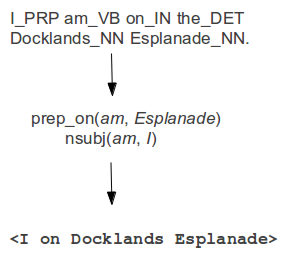
\includegraphics[width=0.5\textwidth]{phase1.png}
\epsfig{file=turnA.eps, height=1.5in, width=1in}
\caption{Ambiguity arises when the route instructions are based on 
standard direction models as \textit{take a left}.}
\label{fig:turnA}
 \end{figure}

 \begin{figure}[htb]
\centering
%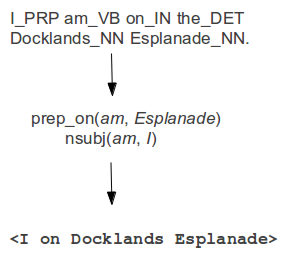
\includegraphics[width=0.5\textwidth]{phase1.png}
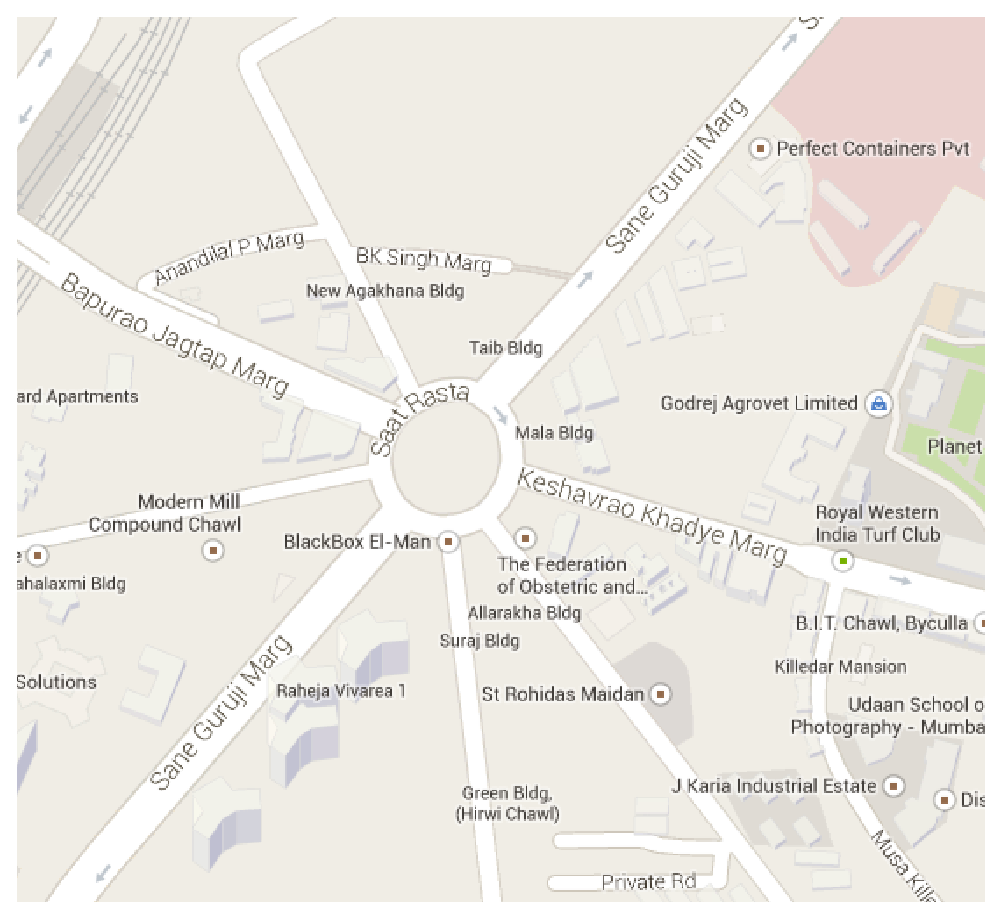
\epsfig{file=complex_real.eps, height=3in, width=3in}
\caption{Real world example of a complex intersection in Mumbai, India 
taken from Google Maps \cite{gmaps}.}
\label{fig:complex_real}
 \end{figure}

The communication protocol proposed is an adaptive approach to formal 
representation of route instructions. It uses a standard direction model 
similar to Klippel \cite{klippel} when the resulting indications are non
-ambiguous. However, if the turns are complex, it uses a clock-based 
convention to represent turn directions. The protocol uses a language 
independent symbolic encoding for landmarks and turn instructions at 
decision points. The two scenarios of simple and complex intersections 
differ in the symbolic encoding of directions while landmarks use their own 
notational representation and below we elaborate on each of these. 

\subsection{Landmarks}
The landmarks are represented by notational IDs and by the direction 
(left or right) in which an user encounters this landmark while moving on 
a path segment. So, if $X$ is the notational ID of a landmark and if 
moving on the directed path segment, the user would encounter $X$ on his 
right, then the corresponding representation is $X^R$. Similarly, $X^L$ 
indicates that moving on the path segment, user can see $X$ on his left. 
These representations along with that of turn behaviour at intersections 
(simple and complex) form the communication protocol. approx

\subsection{Simple Intersections}
Most of the intersections in the real-world fall under this category and 
are fairly trivial to communicate. To formally define a \textit{simple 
intersection}, we divide field-view of the navigator in four triangular 
zones (see Figure \ref{fig:simpleturns}). Choosing reference axis as the 
left direction perpendicular to the incoming road segment $p$, the left 
zone spans 45 degrees on either side of the reference point. Its mirror 
image in the field-view w.r.t. the decision point is the right zone. 
Similarly, one can conceptualize the other two zones. We define a 
decision point as a \textit{simple intersection}, if in each zone of the 
navigator's field view, there is atmost one road segment emerging from 
the decision point. 

The instructions that are associated with change in direction are 
represented by symbols \textbf{R} and \textbf{L}. The non-turning 
instruction indicating that one should go straight is represented by {\bf S}. 

\begin{figure}
\centering
%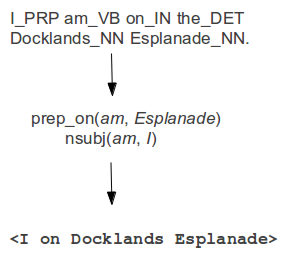
\includegraphics[width=0.5\textwidth]{phase1.png}
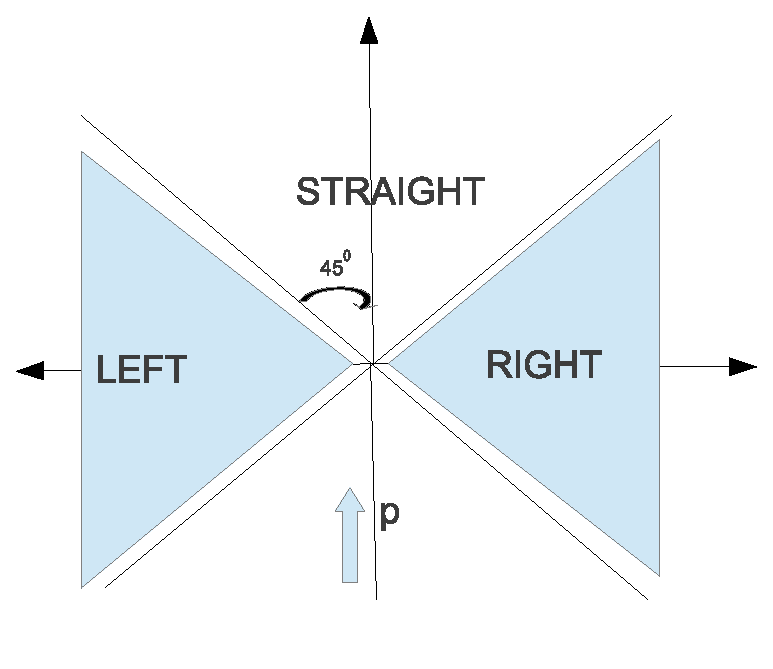
\epsfig{file=simpleturns.eps, height=3in, width=4in}
\caption{A decision point is simple intersection, if in each zone of the navigator's field view, there is atmost one road segment emerging from the decision point.}
\label{fig:simpleturns}
 \end{figure}
\subsection{Complex Intersections}
\begin{figure}
\centering
%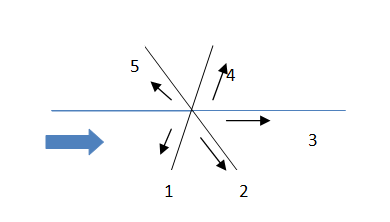
\includegraphics[width=0.5\textwidth]{complex.png}
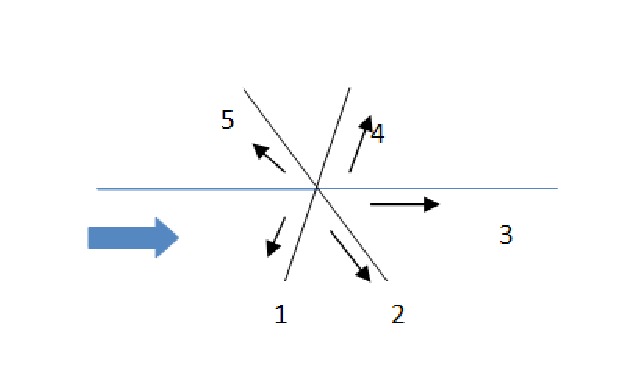
\epsfig{file=complex.eps, height=2.5in, width=5in}
\caption{Clock based convention to non-ambigously represent directions at complex intersections}
\label{fig:complex}
 \end{figure}
\begin{figure}
\centering
%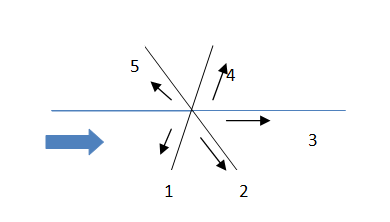
\includegraphics[width=0.5\textwidth]{complex.png}
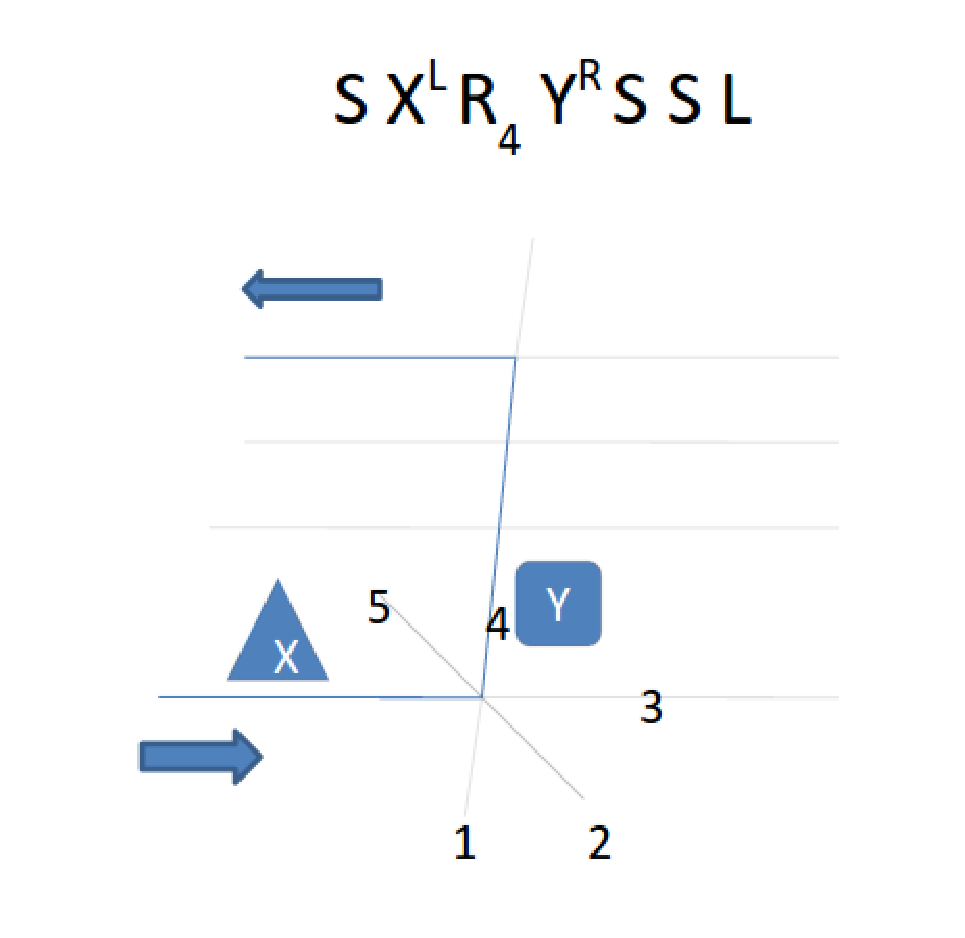
\epsfig{file=complexex.eps, height=3.5in, width=3in}
\caption{An Example to showcase an application of the proposed 
communication protocol. The intended route is represented symbolically in 
text at the top of the image. One possible translation of the encoding in 
english language can be as: 
1. \textit{Go Straight}
2. \textit{You would find X on your left}
3. \textit{At the intersection, take the 4th link in anti-clockwise direction from the most adjacent turn at your right side} 
4. \textit{You would find Y on your right}
5. \textit{Take the third left after Y}
}
\label{fig:complexex}
 \end{figure} 
Any decision point which is not a simple intersection is a 
\textit{complex intersection}\footnote{See Figure \ref{fig:complex_real} 
and Figure \ref{fig:complex}}. For representing complex intersections, we 
use a clock-based notation for a non-ambiguous representation. Klippel 
\cite{klippel} handles non-standard turns by using an 8-sector model which 
opens up alternate notations such as \textbf{hl} (half left), 
\textbf{vr} (veer right), etc. These work well for 4-way intersections 
and 3-way intersections but as the number of merged road segments 
increase beyond 4, the 8-sector model fails as there can be more than one 
road segment in the same sector. A clock-based notation does not work on the 
basis of a sector model and can handle extended multi-way intersections.

There are two ways to conceptualize a clock-based numbering scheme - clockwise and anti-clockwise. A user who is restricted to travel in a clockwise direction around a complex intersection has to be given instructions using the direction of travel as a reference. Thus, a fixed numbering scheme can't work in all scenarios. For example, in India, the direction of travel is clockwise, while in western countries it is anti-clockwise. Hence, we chose to specify whether the numbering is clockwise or anticlockwise at a global level and then let the algorithm make use of it. In the below discussion, we assume the global specifications pertaining to anti-clockwise direction of travel.

The roads are represented in an anti-clockwise numbering starting from the first turn right-adjacent to 
incoming road segment as shown in Figure \ref{fig:complex}. Notationally, 
we represent complex turns in the form $R_i$, which represents the 
$i^{th}$ numbered turn in an anti-clockwise direction starting from the most 
adjacent turn on your right.

Figure \ref{fig:complexex} elaborates a full-fledged example combining 
the representations of landmarks and intersections and attempts to 
present an english translation of the same. Before we conclude, we claim 
that the qualitative calculi used by Klippel \cite{klippel} on formal 
representations can be applied likewise to the proposed communication 
protocol as it directly extends it by including 
complex intersections. So if a route has no complex intersections, our 
communication protocol is semantically similar to that of Klippel. 
Continuing the example from Figure \ref{fig:complexex}, the route 
segment corresponding to the representation $SSL$ is translated as 
\textit{the third left} which is similar to the chunking rule of 
Klippel's \textit{wayfinding choremes} \cite{klippel}, where by the help 
of term rewriting, an intermediate representation is deduced from simple 
representations, prior to natural-language translation.

%We implemented this protocol and incorporated in our testbed to demonstrate the validity and non-ambiguity of its semantics.
 \chapter{Dialog-Based Localization}

In the previous chapter, we proposed a communication protocol to convey 
turn behaviour at every intersection. In this chapter, we introduce the 
algorithm for dialog-based tracking between the intersections to 
determine user's location and temporally align the delivery of route 
instructions with the user's movement and confirm his orientation. While 
posing questions to a user for localization and confirming orientation, 
we propose the use of an alternative reference to landmarks which 
highlights the distinctive geometry features. We next present a method to 
extrapolate movements of a user for location inference using speed 
predictions. To further cope up with errors and misinterpretations, we 
also introduce the algorithms to detect and resolve disorientations. The 
localization alogrithm along with the communication protocol are the 
two mutually exclusive and exhaustive components of the proposed location-
unaware dialog-system. 

\section{Introduction} 
While guiding a user to his next path segment, its required to keep track of the user's location to avoid any disorientation. Since, there is no device-based support for location sensing, the only way to localize a user is by asking him about his location in a controlled input format. Though, researchers \cite{tellex:language, Kordjamshidi:labelling, matuszek:following} have been working on processing unrestricted NL input to extract spatial information but none of these have been able to overcome the classical information extraction errors limiting the output. Further limitations brought by poor speech recognition add to the ineffectiveness of using unrestricted language as input. 
For this work, we try to limit the questions to those with an objective reply (such as yes or no) or recognisable speech commands (such as color of a building, etc.). These questions are strategically based on the salient features of the spatial environment i.e. \textit{landmarks}. The other requirement to provide quality user interface is to be able to predict the correct position of the user with a good enough estimate, such that the number of questions asked to confirm the orientation and localize the user are kept to minimum. The `number of questions asked',as we would discuss later in detail in Chapter \ref{evaluation}, remains as a prime evaluation criteria.

\section{Alternative Reference to Routemarks}
\label{sec:altref}
In any session of wayfinding, a user is incrementally guided for turn behavior at every intersection. Between every two intersections, user is prompted for localization via questions based on whether he encountered the associated landmarks en-route. \footnote{The issue of how landmarks are associated to a path segment are discussed in Section \ref{kbase}.}. Lovelace et al. \cite{lovelace} distinguish between the landmarks according to the purpose they serve i.e. either in choosing the action at a decision point (landmarks) or confirming reorientation on a path segment (\textit{routemarks}). In localization, landmarks are always treated as routemarks and with this, there is a difference in how they are communicated to the user. In the following discussion, the term landmark would be used substitutively for a routemark. 

A landmark is referred to by its name (e.g., Eiffel tower) or by its category (e.g., hospital, T-junction) or both, depending on whichever defines its distinctiveness in its locality. Although, in general category-based landmarks are easily comprehensible under route instructions but similar familiariaty is not guaranteed with name-based landmarks unless the name is explicitly mentioned in a readable form (like for hotels). In such cases, it is preferable to refer a landmark by its distinctive geometry feature (if any or else choose a landmark by geometry). For example, instead of refering to that building as \textit{Visitor's Hostel}, the system should refer it alternatively as the ``red colored 2-floored building'' if its the only one so in the locality. Since, even a category-based landmark can be misinterpreted, esp. when its structure doesn't directly reflect its category (like a movie theatre might not look like a theatre), we reference a routemark by its distinctive geometry feature if its salience falls below a certain threshhold. The threshhold parameter differs for name-based landmarks based on the assumption that the chances of unfamiliarity to a name are more than the mismatch of landmark structure with its category.
\section{Extrapolating User Movements}
\subsection{Estimating User Speed}
Consider the situation when the user is on a particular path segment and is being guided to his destination through an incremental set of instructions. At this point, the instruction pertaining to the next intersection has been made known. The prompts are such that the user is required to give a positive response only when he sees a particular landmark after taking the needed action. For example, natural language equivalent (in English) to such a prompt could be, \textit{Go straight at the next intersection and prompt me `Yes' when you see a cafeteria on your left}. These instructions as discussed earlier are a part of the communication protocol. At this point, if the user follows the instruction correctly and takes a non-turning action at the next intersection, he should see the \textit{cafeteria} on his left after some point of time. Since, the instructions do not explicitly or implicitly mention about any intersection in between, it is guaranteed that between the \textit{cafeteria} and current location of the user, there is exactly one intersection. The time when a positive response is recorded from the user, the \textit{cafeteria} becomes the new current location of the user. Thus based on distance measures and the corresponding time difference, speed can be computed. Thus, speed estimation can be put as:
\[\displaystyle \textit{User Speed}=\frac{\textit{Distance between two recorded prompts}}{\textit{Time difference between the two prompts}}\]
\subsection{Predicting User Speed}
Speed predictions lead to adaptive nature of the localization algorithm and assist in extrapolating movement patterns of a user as per his speed profile. Continuing from the above example, consider a case when user doesn't respond with a `Yes' prompt for a relatively long time. If the system acts passively waiting for the `Yes' prompt, a disoriented user may be totally lost (unless the system accepts unrestricted NL to process a general user query). Thus, there needs to be a predefined time limit in which the user is expected to provide a response. If this time limit expires, the sytem can interrupt to generate another prompt confirming his orientation. Thus, to get an estimate of this time limit, it is required to predict speed of the user. 

The speed predictions are done specific to a road segment and time of day. Some roads facilitate faster speeds than the others but the differences differ over the time of day.
Also to be considered is the speed profile of the user. A slow driver might prefer to drive slow proportionately in every speed-limit scenario. Summing up, the algorithm for speed prediction works over two predictors - 
\begin{itemize}
\item historical average speed on the road segment at this time of day $(H_{e,t})$,
\item average relative speed deviation of the user from the historical speeds $({A_u})$,
\item dynamic slowdown factor (f).
\end{itemize}

For every upcoming road segment, speed is predicted using historical average speeds on the roads and the average deviations of the estimated speed of the user in this session from the historical average speeds on the travelled roads. The feature historical average speeds is stored specific to discretized time slots in a day owing to the observation that a road might be distinctly fast in the late nights as compared to that in peak-hours. The average relative speed deviation feature is related to the characteristic of the user and can help identify driving preferences. This gives a slow driver enough time gap between successive prompts for confirming orientation, while a fast driver might get different prompts to spatio-temporally match his rapid movements.  

The third predictor is meant to consider live traffic information. There may be cases when a road has history of fast vehicle operating speeds and yet, temporary slowdowns maybe observed even for drivers with high-speed driving preferences. Such slowdowns usually occur due to natural interruptions such as foggy weather, torrential rains or snowfall, or even man-made interferences like festival celebrations, rallies or occassional traffic-jams due to miscellaneous reasons. The estimation of dynamic slowdown factor is done freshly at each time slot by averaging relative slowdowns at the given edge from all the users and can be mathematically modelled as:
\[\displaystyle f_{e} = \frac{1}{|U|}\sum_{u \text{ } \in \textit{ U}}(1-\frac{(A_u - A_{e,u})}{A_u})\]  
\begin{align*}
A_{e,u} - \text{speed deviation of user} \textit{ u } at \textit{ e } \text{from historical average speeds at }\textit{e} \text{ at given time slot} \\
A_u - \text{average relative speed deviation of the user \textit{u} from the historical average speeds} \\
U - \text{the set of users who travelled the edge \textit{e} in this time slot} \\
f_e - \text{slowdown factor for edge \textit{e} at given time slot}
\end{align*}
\section{Detecting Disorientation}
As discussed before, exactly one prompt is posed to the user between every two intersection points. This prompt asks the user to confirm his position and is put as early as possible at a road segment to detect disorientation early. There are two cases possible if no response is received from the user within the time limit (set after speed prediction). These cases are handled as below. Algorithm \ref{algo:detect} presents the algorithm to detect disorientation.


\begin{algorithm}[H]
\label{algo:detect}
\SetVline
\dontprintsemicolon
\SetKwInOut{Input}{input}\SetKwInOut{Output}{output}
\Input{Response received at the end of time limit (can be None), \\the landmark position expected and\\ current time limit}
\Output{1, if detected disorientation, 0 otherwise}
\BlankLine

\eIf{response is positive}{
go to next route segment\;
current location becomes this landmark\;
}{
prompt to ask if the intermediate intersection was crossed\;
$response \leftarrow getInput()$  

\eIf{response is positive}{
    $timeFrame \leftarrow timeFrame\times waitFactor$\;
    \tcp{wait for timeFrame}
    $response \leftarrow getInput(timeFrame)$ \tcp{blocks for timeFrame units} 
    \eIf{response received and response is positive}
      {return 0\;}
     {
     \tcp{Here when no response received or negative response}
     return 1\;} 
  }
{return 0\;}
}
\caption{DetectDisorientation(response,landmark,timeFrame)}
\end{algorithm}
\subsection*{Case-I - Slow Driver}
If the user is unable to reach the next position within the expected time frame, then he might not be able to see the instructed landmark before the end of time limit and thus no `Yes' prompt would be received even though the user is not disoriented. Since, it is very much possible to be slow in crossing a intersection esp. if it involves clearing the traffic signals, such cases are duly considered and the system inquires whether the intermediate intersection was crossed. If the answer is `No', then the system delegates the next position to this intermediate intersection and waits for a `Yes' prompt which if received, confirms that the user has crossed the intersection. 

\subsection*{Case-II - Disoriented User}
However, if the system receives a `Yes' prompt at the inquiry for crossing the intersection, it waits for an additional time frame (which is sized as that of the original frame reduced by a wait factor). This additional time frame is used to accomodate possible slowness of the driver assuming that the user though running a little slow would encounter the desired landmark at the next path segment. Once the additional time frame expires and yet the user doesn't see the instructed landmark despite having crossed the intesection, the system traps into the user for reorientation. This situation is depicted in Figure \ref{fig:detect}. 
\begin{figure}
\centering
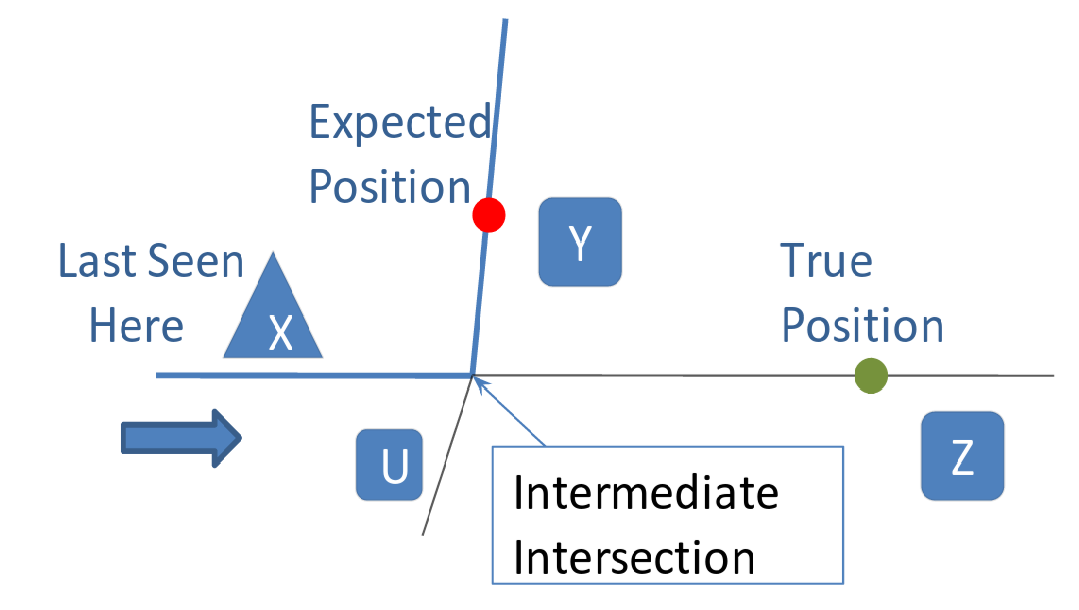
\epsfig{file=disorientation.eps, height=2in, width=3in}
\caption{\textbf{Detecting Disorientation} The highlighted route denotes the path segment communicated to the user for wayfinding. The user has disoriented from the desired path segment and has been detected by the system after a positive response on querying on whether the intermediate intersection was crossed.}
\label{fig:detect}
 \end{figure}
\section{Reorientation algorithm}
\label{sec:reorient}
The process of tackling disorientation is divided into two phases, each with its own characteristic way of causing reorientation. 
\subsection*{Phase-I: Anticipative}
The first phase is \textit{anticipative phase} where we estimate user's position based on movement extrapolation using all possible paths from the last seen point (LSP). The idea is to localize the user to the nearest landmark visited by the user. In the act of localization, the user is prompted with the possible landmarks he could have encountered en-route. For example, consider the case shown in Figure \ref{fig:anticipative}. Once disorientation is detected for the user, then based upon speed predictions for the user, the possible path segments and associated landmarks are identified. Thereafter, we prompt the user with questions identifying these landmarks (\textit{U, V, W} and \textit{Z}) along with the orientations w.r.t. user (left or right) to get the location estimate. Reorientation is achieved when the user acknowledges any of the identities put in the prompts.
\begin{figure}
\centering
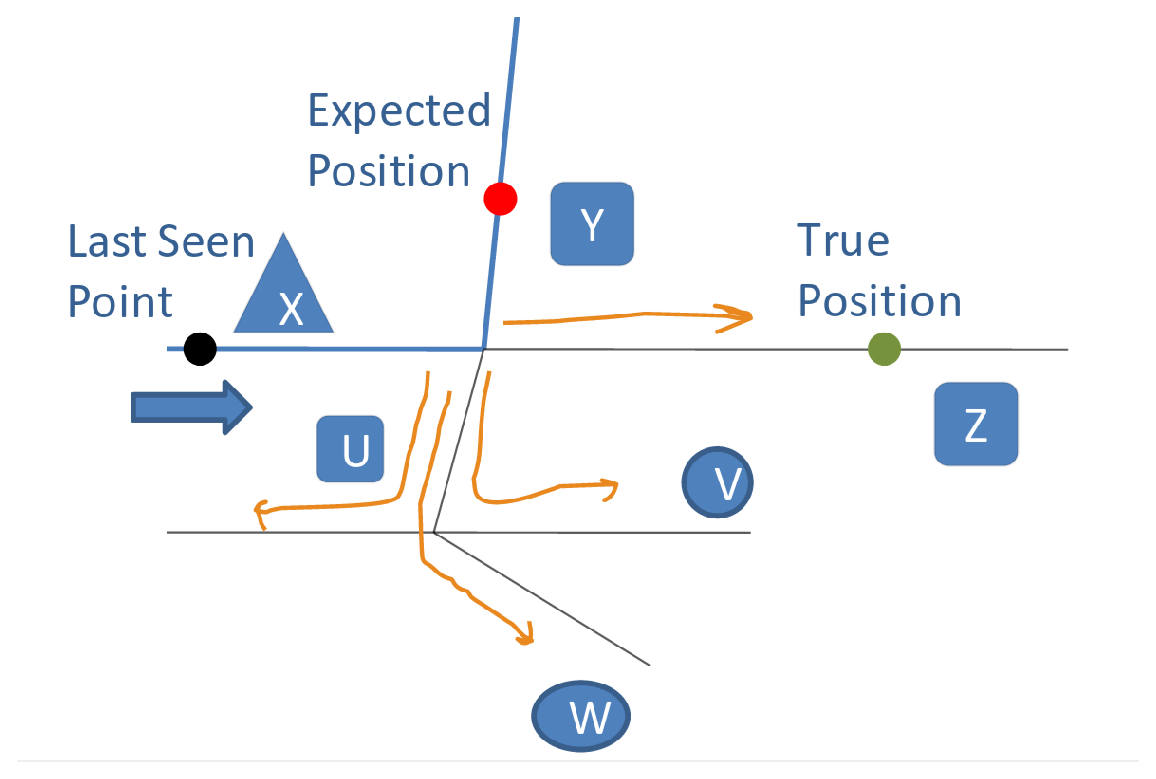
\epsfig{file=reorientationAnticipative.eps, height=2.5in, width=4in}
\caption{\textbf{Reorientation:Anticipative-Phase} Prompt the user with questions identifying landmarks \textit{U, V, W} and \textit{Z} along with the orientations w.r.t. user (left or right) to get the location estimate. Reorientation is achieved when the user acknowledges any of the identities put in the prompts.}
\label{fig:anticipative}
 \end{figure}
\subsection*{Phase-II:Reactive}
In a case where small number of prompts suffice in reorientation, one can directly query for identification over all such landmarks seen on the way. But when the number of prompts increases by more than an acceptable extent, we opt to switch the reorientation strategy. Until now, we were being anticipative and the questions asked were of the form `\textit{do you see U on your right?}'. In the reactive strategy, we attempt to capture the environment of the user by querying over well-defined attributes. For example, the questions now are of the form `\textit{do you see any building nearby?}' The term `\textit{building}' here is one of the categorizing attributes of landmarks which is a part of the feature-set stored as visual features in the knowledge base\footnote{See Section \ref{kbase} for more details}. The feature-set includes attributes like color of the buildings, heights, shapes of the open spaces and other automatically extractable attributes.

The major drawback in solely relying upon the above strategy is that it doesn't guarantee to localize a user and is dependent upon the stored visual features. In some cases, even after exhaustively asking questions on the categorizing attributes, there still might be a set of possible locations of the user. For example, in an ideally homogenous neighborhood, buildings in all streets might look alike in shape, color and height. For such cases, when there are still a set of locations under consideration, the user is asked to follow his original direction of movement only to be interrupted later for yet another reorientation. This process is iteratively repeated until the responses resolve the location of the user distinctively.

The reactive approach is motivated by the \textit{scene analysis} location sensing techniques \cite{hightower}. These techniques work on visual images or electromagnetic measurements to sense observed features of a scene for determining a user's physical location. Understandably, the features used are simple that are easy to represent and compare from an observed scene. The approach mentioned is a hybrid of \textit{static} and \textit{differential} scene analysis. In the former technique, features in question are looked up from a pre-defined geo-spatial database, whereas in the latter, differences in scenes observed with user's movements are used to match known spatial environments.

 \chapter{Implementation}
In chapter 3, we discussed the architecture of a generic wayfinding model, its structure and interaction of the different modules. In this chapter, the implementation-specific aspects of the key components are described with consideration to its application in developing a location-unaware dialog based system. We discuss a methodology to build the knowledge-base by automated extraction of attribute-values and identification of associations in the entities to represent spatial information. Furthermore, in context of reorientation, we introduce our approach to study movement patterns in order to facilitate early localization of a disoriented user.

 \section{Knowledge Base}
  \label{sec:kbase}
A given map dataset can be imported directly into a relational-database model where each shapefile gets converted to an individual relation. The properties of spatial features are converted to attributes and each spatial feature forms a tuple in the relation. The attributes of the spatial features can be divided into four categories:
\begin{itemize}
  \item \textbf{identitificational} - these attributes include \textit{reference-id} as a pointer to the spatial feature, and \textit{category} specifying the class of the spatial feature. The values to category attribute can come directly from the shapefile to which they belong.
  \item \textbf{geometric} - for a spatial database, geometry comes as a primitve datatype. This allows the definition of functions to handle geometry based operations and make several deductions like area, length, etc.
  \item \textbf{visual} -  these attributes define the visual attributes like height of a building, color of a playground, etc.
  \item \textbf{semantic} - these attributes are defined as per external sources can meant to identify the meaning behind a feature e.g., petrol-pump, ATM.  The major attribute that falls in this category is the popularity of the feature as a landmark which facilitates context-aware wayfinding.
\end{itemize}

The first two of these attributes can be defined to be \textit{intrinsic} attributes as these are present or can be easily extracted from exisiting spatial databases. While, the other two attributes are \textit{extrinsic}, as external resources need to be used for their extraction.
\subsection{Extracting Attribute Values}
Raubal and Winter \cite{raubal} worked in a similar research categorising the attributes defining landmarks and provided a methodology to automatically extract local landmarks using integrated datasets such as 3-D city model, navigation graphs and georeferenced images of every house in the neighbourhood. Such an approach offers to improve services giving a with resources on-supply to populate the visual and semantic attributes. But, the research evidently states that to extract visual and semantic features, one needs comprehensive datasets and extrinsic dependence. Brenner and Elias \cite{brenner} focussed on extracting the landmarks structurally using data mining on spatial databases. The approach focusses more on intrinsic attributes (such as form factor of a building, distance off the road segment,etc.), values of which are extractable on processing from the map itself but also highlight the use of laser methods to identify certain visual features (such as height, visibility). The various attributes considered in their work to extract salient landmarks are shown in Figure \ref{fig:elias}.

We opted to work on the lines similar to \cite{brenner} to define the geometric salience of buildings. In a real-world application, only those attributes should be considered that are identifiable and communicable. For example, \textit{form of parcel} (in Figure \ref{fig:elias}) might be a difficult attribute to realize in English language and equally difficult to be identified by a driver. On the other hand, \textit{road distance} is easily identifiable and communicable. Apart from the buildings, we also considered open spaces (such as playgrounds or parks) while searching for salient features in a neighborhood. Though a street may well be surrounded by structurally similar buildings but a large enough open-space area in it would be sufficient to confirm orientation of the user if there is no such feature in the neighbouring streets. We do not rely upon the visual and semantic attributes of a landmark for two reasons: (a) the geodatasets used for extracting such information are scarce and limited, and (b) the requirement of our guidance algorithm from the attributes of a landmark is fulfilled if they can make the landmark uniquely identifiable in its local neighborhood. Though visual and semantic attributes would enhance the identifiability but the algorithm is adaptive to the absence of such attributes. We tested the usage of such attributes in guidance and localization using synthetic settings wherein the number of available attributes was parametrized and attribute values were randomly assigned.

\begin{figure}
\centering
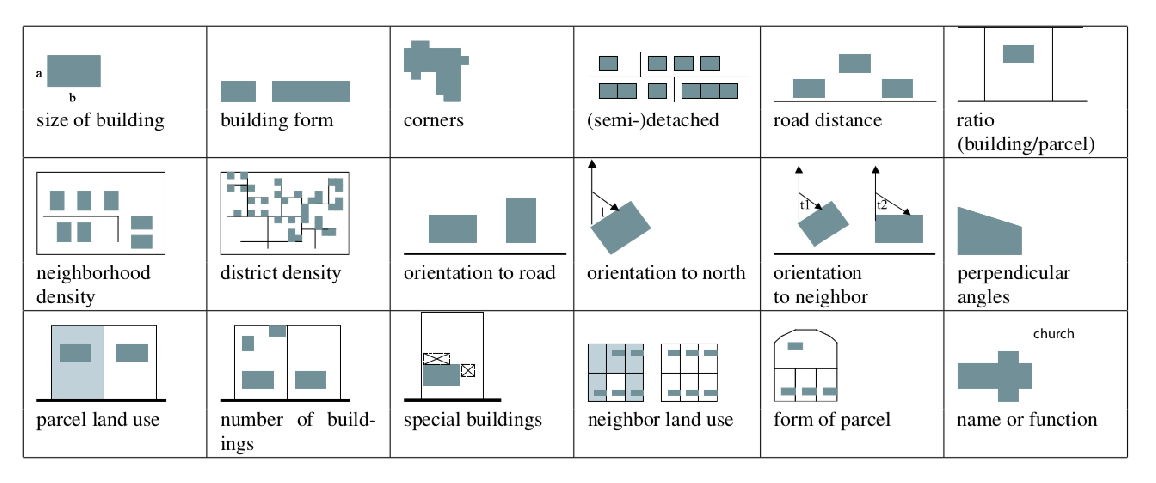
\epsfig{file=brenner.eps, height=2in, width=6in}
\caption{\textbf{Extracting Geometric Salience} The geometric attributes used by Brenner and Elias \cite{brenner} to extract building-based landmarks}
\label{fig:elias}
 \end{figure}

Semantic attributes pose a challenge for automated extraction and demand for sophisticated web-mining approaches for qualitative results. Tezuka and Tanaka \cite{tezuka} present one such approach of exploiting world wide web to extract landmarks from digital documents with good precision. However for the purpose of this work, we used a simple and a scalable approach to extract semantic attribute of \textit{popularity} using web resources in order to enhance feature identifiability wherever possible. The popularity of a landmark can help in deducing familiarity of a navigator\footnote{Also, see Section \ref{sec:altref}}. For example, if a user comprehends instructions which refer to less popoular landmarks by name, it can be assumed that he is well-familiar with the neighborhood and thus, instead of using geometric features for making a landmark identifiable, the local names of the landmark can be used for wayfinding assistance. The extraction methodology exploits two well-known mapping applications as resources Google maps \cite{gmaps} and Wikimapia \cite{wiki}\footnote{depicted in Figure \ref{fig:popular}} and is described below.  Also, since these applications also collect metadata in the form of user-reviews, they can be utilized to obtain local-names/alias for the spatial features of an environment which are not present in traditional geodatabases.
\subsubsection*{Using Google Maps}
To help provide development services, Google-Maps provides a ranking scheme to search for popular places in nearby area via its Places API. The ranking scheme utilizes the quality of citations and reviews to places done by its extensively large user base. The search results show upto 60 places ranked in the order of prominence for a given query for a given radius. Thus it forms a convenient application to find popular places in a neighborhood or equivalently to find popularity of a given location as compared to its local neighborhood. We applied this methodology to IITK campus and exploited the results of the search to contribute to the \textit{popularity} attribute. Due to a comparatively small area occupied by the campus, the attributes were populated with a single search query with radius set to 2km from PK Kelkar Library, the approximate center of IITK campus.

\subsubsection*{Using Wikimapia}
Unlike Google Maps, wikimapia is an open-content mapping application and it provides free access to its extensive geodatabase. The maps in wikimapia are edited and updated via crowdsourcing. And again, unlike Google, it doesn't provide any ranking index to directly find the prominence of a location. But, it does provide an open access to all the reviews submitted for the places in its spatial database. Based on the heuristic that a popular place would have a comparatively large number of reviews submitted, we extract and map popularity to the corresponding locations using the number of reviews as values. Under wikimapia, we define popularity of an area as the total number of reviews submitted of all places enclosed under it.
\begin{figure}
\centering
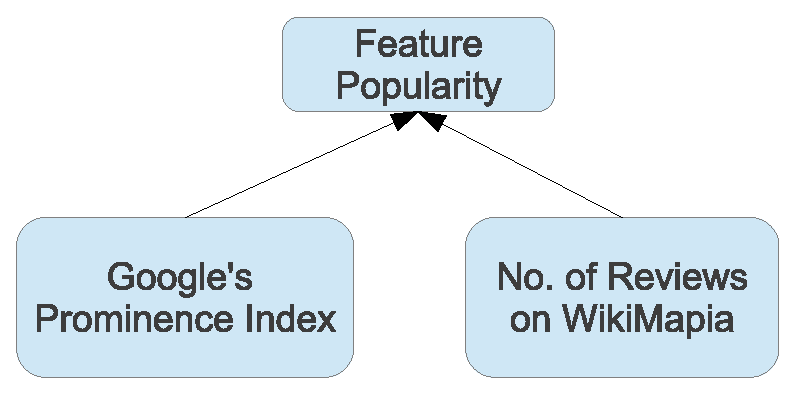
\epsfig{file=popular.eps, height=1.5in, width=2in}
\caption{\textbf{\textbf{Extracting Popularity}} A scalable approach to get an indication on the popularity of a landmark using dependence on mapping applications.}
\label{fig:popular}
 \end{figure}

\subsection{Identifying associations}
Having combined the resources for extracting attribute values in building relations for the features of an environment, the need is to provide an interface to use this spatial information in a real-time wayfinding assistance task. To be able to use the features in route instructions, every road segment needs to be associated with a certain feature (landmark) which serves to confirm the orientation of a user. For the purpose of this work, we used nearness heuristic based on the closest distance between the landmark and the road to identify the association between a landmark and a road segment. The distance threshholds qualifying a landmark's association are chosen to be minimum so as to allow identifiablity of attributes by a driver. 

If visibility analysis methods are available (3D models, laser scanning, etc), distance criteria can't be relaxed beyond a certain extent as even though a landmark is visible from the road segment but it can't be guaranteed that the attributes of the landmark can be identified by a distant driver. Also, as per Lynch \cite{lynch}, distant landmarks are used only for overall guidance by novice.

\section{Facilitating Reorientation}
In Section \ref{sec:reorient}, we discussed the algorithm to reorient a disoriented user by querying over possible paths. Trajectory predictions can assist in reorientation by studying distraction patterns which can be exploited for faster localization. These patterns may arise due to environmental factors, complexity of the underlying communication protocol or arbitrary human errors. Trajectory prediction algorithms have been previously developed for improving QoS in cellular mobile networks (\cite{kyri}) and facilitating location based services by predicting future locations (\cite{karimi}). These situations differ from the context of disorientation in wayfinding in which the movements are biased based upon route instructions. 

The approach for our trajectory prediction is bases on probabilistic modelling of movements under the constraints of route-instructions and extends the constraint-free modelling approach adopted in \cite{liu}. The model calculates probability of disorienting on a particular road segment ($Y$) from the given path segments ($X,I$). To realize the model, the required probability is output from a conditional probability $P(Y/X,I)$ which can be put as
%
$$D_{S_1,R_1,R_2} = P(Y=S_1/X=R_1,I=R_2)$$
%
where $S_1,R_1$ and $R_2$ are road segments and $D_{S_1,R_1,R_2}$ is the probability to disorient to road segment $S_1$ when the user is currently on $R_1$ and instructed to move next to $R_2$. The probability is estimated based on historical movement patterns and can be formulated as
%
\[ \displaystyle P(Y/X,I) = \frac{N(Y/X,I)}{ \mathlarger{\sum}\limits_{y \in O_{X,I}} N(y/X,I)} \] 
%
where $O_{X,I}$ is the set of all the road segments at the intersection of $X$ and $I$, and $N(y/X,I)$ is the number of times road segment $y$ has been taken from $X$ when the next instruction was to take $I$. 

Thus, reorientation algorithm sorts the road segments in decreasing order of probability to disorient to, and prompts them incrementally to the user until a positive acknowledgement is received or limit to the number of prompts is exceeded after which it enters into reactive phase.

\iffalse
$$
\begin{bmatrix}
P(X_2=R_1/X_1=R_1,I=R_1) & P(X_2=R_1/X_1=R_1,I=R_1) & \cdots & P(X_2=R_1/X_1=R_1,I=R_1)\\
P(X_2=R_1/X_1=R_1,I=R_1) & P(X_2=R_1/X_1=R_1,I=R_1) & \cdots & P(X_2=R_1/X_1=R_1,I=R_1)\\
\vdots& \vdots& \cdots& \vdots\\ 
P(X_2=R_1/X_1=R_1,I=R_1) & P(X_2=R_1/X_1=R_1,I=R_1) & \cdots &P(X_2=R_1/X_1=R_1,I=R_1)\\
\end{bmatrix}
$$
\fi
 \chapter{Evaluation}
This chapter describes an intrinsic evaluation of our proposed model, particularly focussing on the ability to localize and reorient a disoriented user. The evaluation is conducted by modelling user behavior with paramters to characterize speed profile and erroneous behaviour. We then measure the performance of the guidance algorithm under a dialog-based interface with regards to quality of user experience. To our knowledge, there has not been any previous work using a virtual user model for evaluating wayfinding guidance. 
 
 \label{evaluation}
 \section{Dataset}
We begin by describing the dataset for our prototype implementation. The dataset used for implementation of the model was taken from the geospatial data of Indian Institute of Technology, Kanpur (IITK). The raw data consists of shapefiles representing different layers of a GIS including road network, geometry and metadata of spatial features such as academic buildings, residential area, parks, etc. Visually, the IITK environment depicts a mix of regions which are variably dense in terms of landmark density (Figure \ref{fig:dataset}. On one hand, the academic area is filled with a plethora of distinct features which can be easily identified by an unfamiliar navigator and residential regions on the other, have almost no salient landmark or mutually distinguishing features. The academic area is built on a dense street network while there are long and clear demarcations in the residential areas
\footnote{Prior to building the knowledge-base, a preliminary processing is done on the road network data. Since the shapefiles for road network are in raw geo-vector format, they need to be converted to routable network for route computations. The road segments are split at intersections to disjoint edges, each with a start and an end node.}.
\begin{figure}
\centering
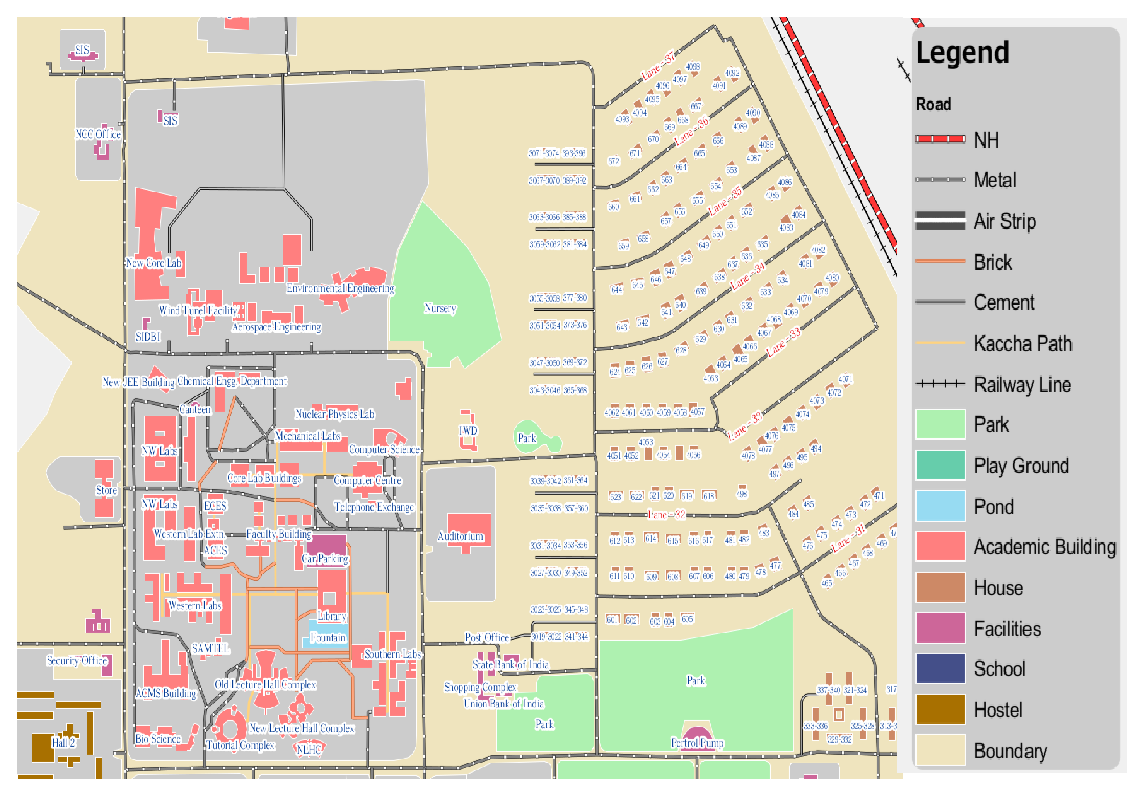
\epsfig{file=iitkmap.eps, height=2.5in, width=4in}
\caption{\textbf{\textbf{Dataset}} Snapshot of the map of Indian Institute of Technology, Kanpur (IITK). The left portion of the snapshot depicting academic buildings (see legend) represents the landmark-dense portion of the campus, Academic area. The organized homogenous space to the right of it represents a portion of the residential areas which has saliently insignificant features.}
\label{fig:dataset}
 \end{figure} 
 \section{Simulation Setup} 
The time spent in executing real-time wayfinding tasks limits the scope of comprehensive testing of a wayfinding-assistance framework. Furthermore, simulations help in situation modelling which has vital importance in studying scenarios of disorientation. The simulation rests on a virtual user model and a synthetic set of feature attributes. The user model simulates varying speed patterns with regards to human behaviour, while the synthetic attribute-set models the extent of diversity in spatial enviroments.
  \subsection{User Modelling}
  \subsubsection*{Speed Profiles}
The speed of a driver at a particular road segment is modelled using two parameters- 1) \textit{categorical-speed} parameter, to represent the speed preferences of a driver and, 2) \textit{deviation} parameter, to add an element of non-uniformity to speed w.r.t different road segments.

%The categorical-speed parameter of a driver is high for users with fast driving preferences and low for those with slow driving preferences. 
The categorical-speed for the drivers are picked from a continuous probability distribution model. Previous studies (\cite{leong,mclean}) have found the normal distribution to work under homogenous traffic flow (same type of vehicles) with moderate to low traffic volume conditions. However under heterogenous traffic conditions, researchers have proposed using a log–normal distribution (\cite{gerl}) for traffic modelling. The log-normal distribution used for sampling categorical-speed is shown in Figure \ref{fig:logn}. The parameters of the distributions are set such that 85th percentile speed is equal to the 30 kph i.e. speed limit at IITK campus\footnote{This is in accordance with the observed relationship between vehicle operating speeds and posted speed limits.} . The deviation parameter is sampled at each road segment from a normal distribution ($\mu=0 kph$, $\sigma=5 kph$) and added to the categorical-speed to generate observed average speed at the road segment.
  \subsubsection*{Erroneous Behaviour}
To cause disorientation in following wayfinding instructions, we modelled a simple error-making probability model of a user which governs user-behaviour at every decision point by choosing each decision with uniform probability. A more sophisticated error-making model would bias decisions based on the structure of the intersection. For instance, one may assign higher probability to go straight when asked to turn left (or right). This may be particularly useful in complex intersections where it maybe difficult to follow route instructions and comprehend in a degenerate natural-language translation of the clock-based convention model.
  \subsection{Synthetic Attributes}
We had discussed possible approaches to extract attributes of a spatial feature in Section \ref{sec:kbase}.  Although since the focus of this work was on dialog-based localization, we chose to synthetically populate the attribute-set of the features. The number of attributes was paramterized in the testbed and the corresponding values were assigned randomly from a fixed set. The idea was to visualize dependency of performance of the localization algorithm on the presence of extrinsic attributes. 
 \section{Goodness Metric}
The major concern with any wayfinding assistance is the extent of interference it causes to the wayfinder. Thus, quality of user experience in a dialog-based wayfinding system would have major dependence on the number of prompts made while assisting to the user. As the complexity of routes increase in terms of number of decisions to be made en-route, greater number of prompts have to be put to the user. Also, if the user commits an error of judgement in following the route instructions and disorients from the intended path, additional prompts need to be put in order to reorient the user. 

Based on the above discussion, we define \textit{goodness} for the evaluation of the proposed model with the metric as number of prompts made to the user ($N_p$) normalized over the total number of decisions made ($N_D$) and, the total number of disorientations ($N_e$) recorded before reaching the destination. The goodness metric ($G$) is formulated as: 
\[\displaystyle G = \frac{N_p - \alpha \times N_D}{N_e}\]  
where $\alpha$ is a constant, representing the number of prompts made in guiding a user on a route with exactly one decision point.
 \section{Results}
 \chapter{Conclusion and Future Work}
\bibliographystyle{plain}
\bibliography{references}
%\addcontents{toc}{bibliography}
\end{document}
